\documentclass[noauthor,nooutcomes,12pt,hints,handout]{ximera}

\graphicspath{  
{./}
{./whoAreYou/}
{./drawingWithTheTurtle/}
{./bisectionMethod/}
{./circles/}
{./anglesAndRightTriangles/}
{./lawOfSines/}
{./lawOfCosines/}
{./plotter/}
{./staircases/}
{./pitch/}
{./qualityControl/}
{./symmetry/}
{./nGonBlock/}
}


%% page layout
\usepackage[cm,headings]{fullpage}
\raggedright
\setlength\headheight{13.6pt}


%% fonts
\usepackage{euler}

\usepackage{FiraMono}
\renewcommand\familydefault{\ttdefault} 
\usepackage[defaultmathsizes]{mathastext}
\usepackage[htt]{hyphenat}

\usepackage[T1]{fontenc}
\usepackage[scaled=1]{FiraSans}

%\usepackage{wedn}
\usepackage{pbsi} %% Answer font


\usepackage{cancel} %% strike through in pitch/pitch.tex


%% \usepackage{ulem} %% 
%% \renewcommand{\ULthickness}{2pt}% changes underline thickness

\tikzset{>=stealth}

\usepackage{adjustbox}

\setcounter{titlenumber}{-1}

%% journal style
\makeatletter
\newcommand\journalstyle{%
  \def\activitystyle{activity-chapter}
  \def\maketitle{%
    \addtocounter{titlenumber}{1}%
                {\flushleft\small\sffamily\bfseries\@pretitle\par\vspace{-1.5em}}%
                {\flushleft\LARGE\sffamily\bfseries\thetitlenumber\hspace{1em}\@title \par }%
                {\vskip .6em\noindent\textit\theabstract\setcounter{question}{0}\setcounter{sectiontitlenumber}{0}}%
                    \par\vspace{2em}
                    \phantomsection\addcontentsline{toc}{section}{\thetitlenumber\hspace{1em}\textbf{\@title}}%
                     }}
\makeatother



%% thm like environments
\let\question\relax
\let\endquestion\relax

\newtheoremstyle{QuestionStyle}{\topsep}{\topsep}%%% space between body and thm
		{}                      %%% Thm body font
		{}                              %%% Indent amount (empty = no indent)
		{\bfseries}            %%% Thm head font
		{)}                              %%% Punctuation after thm head
		{ }                           %%% Space after thm head
		{\thmnumber{#2}\thmnote{ \bfseries(#3)}}%%% Thm head spec
\theoremstyle{QuestionStyle}
\newtheorem{question}{}



\let\freeResponse\relax
\let\endfreeResponse\relax

%% \newtheoremstyle{ResponseStyle}{\topsep}{\topsep}%%% space between body and thm
%% 		{\wedn\bfseries}                      %%% Thm body font
%% 		{}                              %%% Indent amount (empty = no indent)
%% 		{\wedn\bfseries}            %%% Thm head font
%% 		{}                              %%% Punctuation after thm head
%% 		{3ex}                           %%% Space after thm head
%% 		{\underline{\underline{\thmname{#1}}}}%%% Thm head spec
%% \theoremstyle{ResponseStyle}

\usepackage[tikz]{mdframed}
\mdfdefinestyle{ResponseStyle}{leftmargin=1cm,linecolor=black,roundcorner=5pt,
, font=\bsifamily,}%font=\wedn\bfseries\upshape,}


\ifhandout
\NewEnviron{freeResponse}{}
\else
%\newtheorem{freeResponse}{Response:}
\newenvironment{freeResponse}{\begin{mdframed}[style=ResponseStyle]}{\end{mdframed}}
\fi



%% attempting to automate outcomes.

%% \newwrite\outcomefile
%%   \immediate\openout\outcomefile=\jobname.oc
%% \renewcommand{\outcome}[1]{\edef\theoutcomes{\theoutcomes #1~}%
%% \immediate\write\outcomefile{\unexpanded{\outcome}{#1}}}

%% \newcommand{\outcomelist}{\begin{itemize}\theoutcomes\end{itemize}}

%% \NewEnviron{listOutcomes}{\small\sffamily
%% After answering the following questions, students should be able to:
%% \begin{itemize}
%% \BODY
%% \end{itemize}
%% }
\usepackage[tikz]{mdframed}
\mdfdefinestyle{OutcomeStyle}{leftmargin=2cm,rightmargin=2cm,linecolor=black,roundcorner=5pt,
, font=\small\sffamily,}%font=\wedn\bfseries\upshape,}
\newenvironment{listOutcomes}{\begin{mdframed}[style=OutcomeStyle]After answering the following questions, students should be able to:\begin{itemize}}{\end{itemize}\end{mdframed}}



%% my commands

\newcommand{\snap}{{\bfseries\itshape\textsf{Snap!}}}
\newcommand{\flavor}{\link[\snap]{https://snap.berkeley.edu/}}
\newcommand{\mooculus}{\textsf{\textbf{MOOC}\textnormal{\textsf{ULUS}}}}


\usepackage{tkz-euclide}
\tikzstyle geometryDiagrams=[rounded corners=.5pt,ultra thick,color=black]
\colorlet{penColor}{black} % Color of a curve in a plot



\ifhandout\newcommand{\mynewpage}{\newpage}\else\newcommand{\mynewpage}{}\fi


\author{Bart Snapp}

\title{Line art and symmetry}

\begin{document}
\begin{abstract}
  We use lines to draw shapes with dihedral symmetries.
\end{abstract}
\maketitle

\begin{listOutcomes}
\item Find equally spaced points on a circle with sine and cosine.
\item Connect envelopes of tangents to create a shape with regular
  dihedral symmetry.
\item Use and understand a FOR loop.
\end{listOutcomes}

\mynewpage






\begin{question}
  EXPLAIN WHY if I plot the points
  \[
  (r\cdot\sin(i\cdot 360/17), r\cdot \cos(i\cdot 360/17))
  \]
  for $i=0,1,2,\dots, 16$, I'll get $17$ equally spaced points on a
  circle of radius $r$.
  \begin{hint}
    Think of this picture of a triangle on a unit circle:
    \begin{center}
      \begin{tikzpicture}[geometryDiagrams]
        \coordinate (A) at (0,0);
        \coordinate (B) at (0,2.5);
        \coordinate (C) at (4.33,2.5);
        \tkzDrawSegment[line width=2pt](A,B)
        \tkzDrawSegment[line width=2pt](A,C)
        \tkzDrawSegment[line width=2pt](C,B)
        \tkzLabelSegment[below right](A,C){$1$}
        \tkzLabelSegment[left](A,B){$\cos(\theta)$}
        \tkzLabelSegment[above](B,C){$\sin(\theta)$}
        
        \coordinate (xmin) at (-6,0);
        \coordinate (xmax) at (6,0);
        \coordinate (ymin) at (0,-6);
        \coordinate (ymax) at (0,6);
        
        \tkzDrawSegment[->](xmin,xmax)
        \tkzDrawSegment[->](ymin,ymax)
        
        \tkzMarkRightAngle[thin](A,B,C)
        \tkzDrawCircle[dashed](A,C)
        \tkzMarkAngle[mark=,size=1cm,thin](C,A,B)
        \tkzLabelAngle[pos=.7](C,A,B){$\theta$};
      \end{tikzpicture}
    \end{center}
  \end{hint}

  
  \begin{freeResponse}
    This will draw $17$ equally spaced points on the circle, as if we scale the picture above by a factor of $r$, we get:
    \begin{center}
      \begin{tikzpicture}[geometryDiagrams]
        \coordinate (A) at (0,0);
        \coordinate (B) at (0,2.5);
        \coordinate (C) at (4.33,2.5);
        \tkzDrawSegment[line width=2pt](A,B)
        \tkzDrawSegment[line width=2pt](A,C)
        \tkzDrawSegment[line width=2pt](C,B)
        \tkzLabelSegment[below right](A,C){$r$}
       % \tkzLabelSegment[left](A,B){$\cos(\theta)$}
       % \tkzLabelSegment[above](B,C){$\sin(\theta)$}
        \tkzDrawPoint(C)
        \tkzLabelPoint(C){$(r\cdot \sin(\theta),r\cdot \cos(\theta)$}
        
        \coordinate (xmin) at (-6,0);
        \coordinate (xmax) at (6,0);
        \coordinate (ymin) at (0,-6);
        \coordinate (ymax) at (0,6);
        
        \tkzDrawSegment[->](xmin,xmax)
        \tkzDrawSegment[->](ymin,ymax)
        
        \tkzMarkRightAngle[thin](A,B,C)
        \tkzDrawCircle[dashed](A,C)
        \tkzMarkAngle[mark=,size=1cm,thin](C,A,B)
        \tkzLabelAngle[pos=.7](C,A,B){$\theta$};
      \end{tikzpicture}
    \end{center}
    where $\theta = i\cdot 360/n$. So when $i=0$, we start at the top,
    move clockwise around and end back at the top.
  \end{freeResponse}
\end{question}

\mynewpage





\begin{question}
  Here is a STAGE from \snap\
  \begin{center}
    \fbox{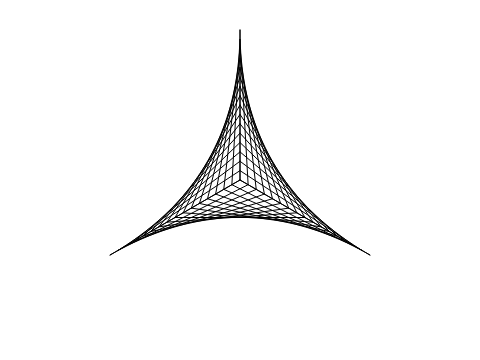
\includegraphics[width=.3\textwidth]{triEnvStage.png}}
  \end{center}
  Use this SCRIPT below to produce the stage above. 
    \begin{center}
    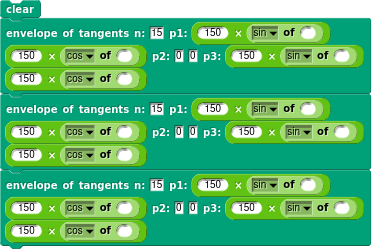
\includegraphics{triEnvScriptBLANK.png}
    \end{center}
    YOU will need to fill in the BLANKS.  In your answer, please show
    off your work with your SCRIPT and your STAGE.
  \begin{freeResponse}
    Here is my SCRIPT and my STAGE:
    \begin{center}
    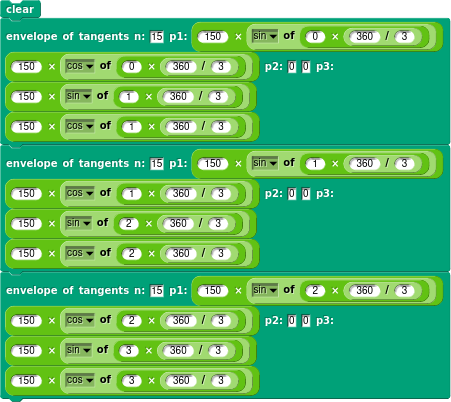
\includegraphics[width=.3\textwidth]{triEnvScript.png}\qquad\fbox{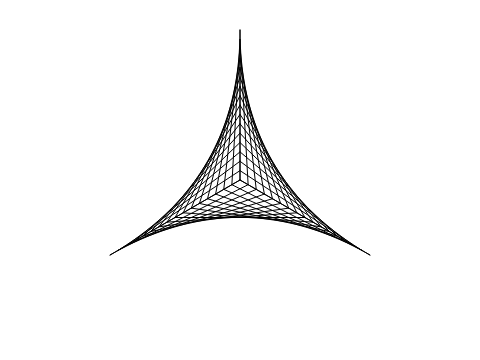
\includegraphics[width=.3\textwidth]{triEnvStage.png}}
  \end{center}
  \end{freeResponse}
\end{question}

\mynewpage


\begin{question}
  We can automate our drawing with a FOR BLOCK:
  \begin{center}
    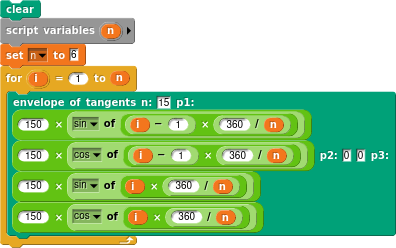
\includegraphics{forEnvTan.png}
  \end{center}
  \begin{enumerate}
  \item Explain the SCRIPT above BLOCK-BY-BLOCK.
  \item Use and MODIFY the script above, to make an ARTISTIC
    IMAGE. Show off your work with your SCRIPT and your STAGE.
  \end{enumerate}
  \begin{freeResponse}
    \begin{enumerate}
    \item \begin{enumerate} We start by making a variable called $n$,
      and we set it to $6$.
    \item Next we let $i$ run from $1$ to $n$.
    \item For each of these numbers we plot an envelope of tangents,
      making a little triangle in a circle of radius $r$.
    \end{enumerate}
    \item Here is my SCRIPT and my STAGE:
      \begin{center}
    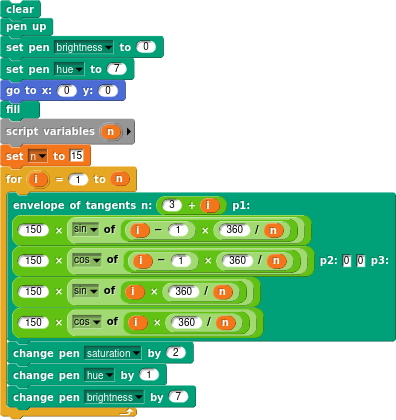
\includegraphics[width=.3\textwidth]{lineArtisticScript.png}\qquad\fbox{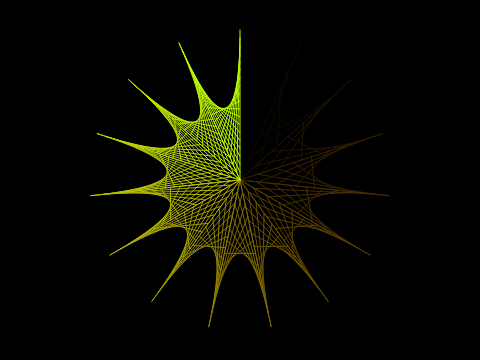
\includegraphics[width=.3\textwidth]{lineArtisticStage.png}}
  \end{center}
    \end{enumerate}
  \end{freeResponse}
\end{question}
\end{document}
